\documentclass[12pt]{article}
\usepackage[margin=1in]{geometry}
\usepackage{indentfirst}
\usepackage [english]{babel}
\usepackage [autostyle, english = american]{csquotes}
\MakeOuterQuote{"}
\usepackage{graphicx}
\usepackage{amsmath}
\usepackage{tikz}

\begin{document}


\title{\textbf{Cloud Computing Simulation for Smart Grid}}
\author{Hanlin Chen\\the Department of Electrical and Computer Engineering\\Ohio State University\\ chen.8059@buckeyemail.osu.edu}
\maketitle 

\section{Introduction}
The growth of power  data in smart gird motivates use of high performance cloud computing  application. In the cloud model, all data processing, software and hardware are delivered to users via internet in forms of service such as platform as a service (Paas), software as a service (Saas) and infrastructure as a service (Iaas). Compared to traditional computing framework, the cloud computing can handle much higher volume of data from smart grid and provide promising power management to users. The performance of cloud model could be addressed by its processing speed and throughput. In addition, various factors such as hardware infrastructures, allocation of virtual environment and smart grid application are directly linked to these performance measurements. In this paper, we proposed a novel cloud based data center architectures to improve data processing in the smart power grid. 
The runtime simulation is done to investigate the effect of hardware configuration and allocation policy on execution of smart grid application using open source toolkit Cloudsim \cite{ok}. The structure of this paper is as follow. Section II reviews overall architectures of proposed cloud based data center for smart grid. Section III studies two common VM scheduling: time shared policy and space shared policy. Section IV includes all simulation results and time analysis. Section V gives the conclusion. 

\section{Cloud-Based Data Center Architectures}

The basic cloud architectures enable supports for maximizing the availability and increasing demand of computing power and data storage\cite{ok2}. In our experiment, the cloud computing service is provided by one power company. Therefore, only 1 Cloud Service Provider (CSP) or 1 data center is required in our simulation. The data center is accountable for providing seamless infrastructure services for all cloud users in the city. In order to achieved higher utilization of computing, the virtualization of hardware is used and allocating computing hardware on user's request. The advantage of virtualization is that the service provider is not obligated to allocate all  hardware resources in advance and charge users based on usage of storage and bandwidth. In addition, it can also prevent applications from interrupting each other during execution, and provide higher data security. The detail of cloud-based data center architectures are displayed in figure 1.

\begin{figure}[ht!]
\centering
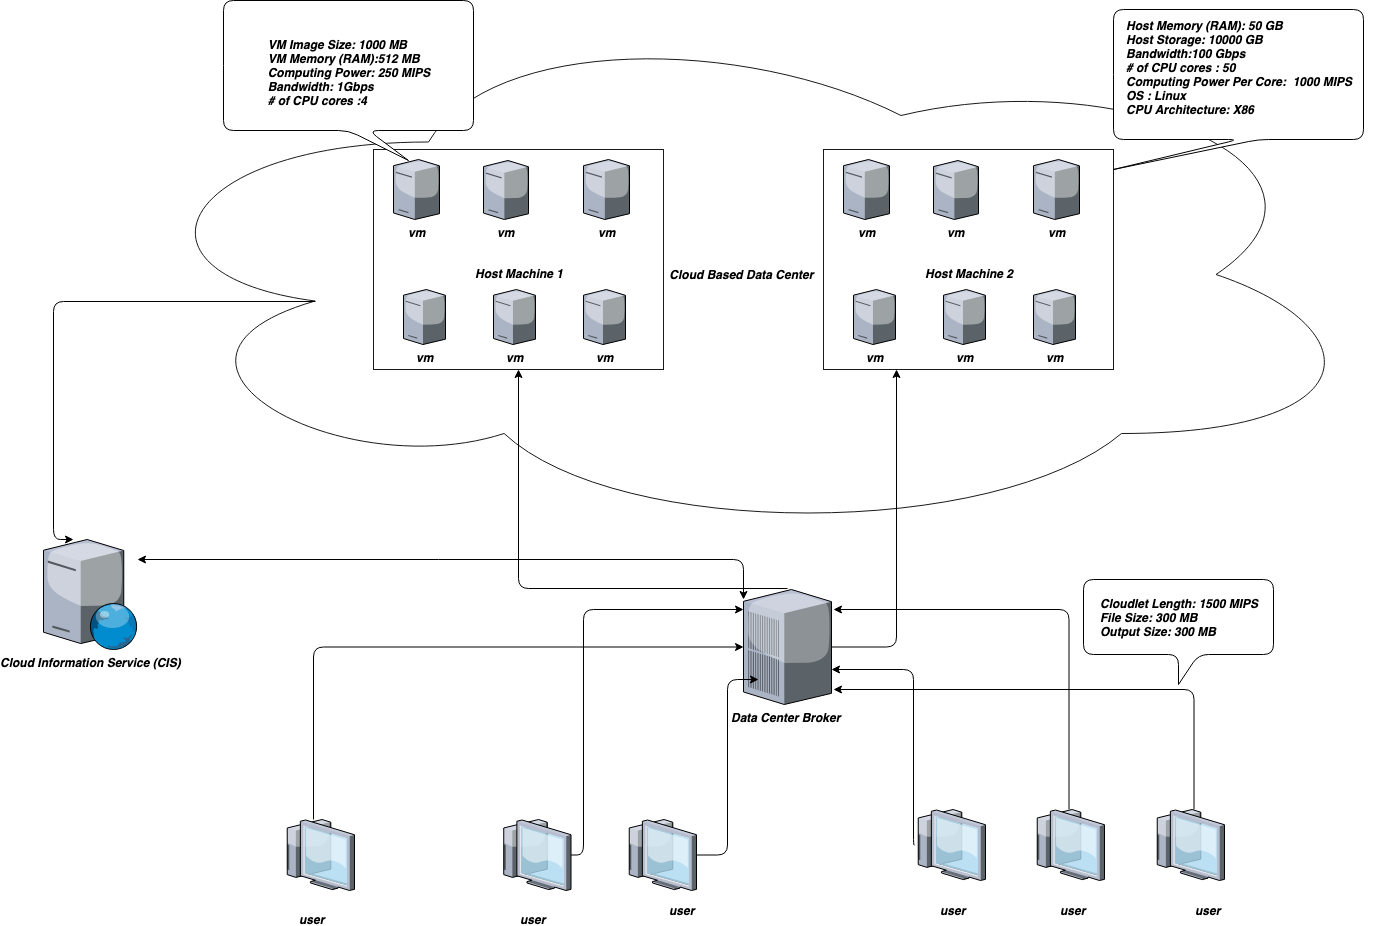
\includegraphics[scale=0.3]{Smart_Grid_Cloud.png}
\caption{The Smart Grid Cloud Architecture}
\end{figure}

\indent The data center has two host machines or servers and each host has the configuration: RAM = 50 GB,  storage  = 10000 GB , bandwidth = 10 Gbps and  2500 CPU cores with processing power of 250 MIPS per core.  We divide the city where has 30000 users into 50 regions and each region is served by 1 VM.  Therefore, number of VM is equal to 50.  Each VM has the configuration: image size = 1000 MB, RAM= 512 MB and 100 CPU cores with processing power of 250 MIPS per core. The total storage and processing power of two host should be larger enough to handle all data  generated from these 50 regions.  The cloudlet is the  job or task that users submit to cloud for processing and has fixed instruction length and data transfer size. For simplicity, in our simulation all user submit cloudlets with same configuration: length = 1500 MIPS , file size = 300 MB and output size = 300 MB.
\indent As shown in figure 1, users submit the cloudlets to cloud for processing via data center broker.  The broker search status of all computing resource and data center characteristics that previously registered by data center in cloud information service (CIS), then allocate virtual machines in the hosts to process cloudlets. After all cloudlets is completed, the broker destroys all allocated VMs.

\section{Time-shared and Space-Shared Allocation Policy}
Since the intuition of cloud provider is to grow company profit by maximizing user's satisfaction. The effective allocation of resources and tasks is key factor to improve user's experiences. Cloudsim provides time-shared allocation and space-shared allocation policies at both host level and VM level.  These two policies works similar to First Come
First Served (FCFS) and Round Robin (RR) algorithms\cite{ok3}. At the host level, the host machine allocate processing power for each VM.  At the VM level, the the VM allocated processing power for each cloudlet.  When the time-shared policy is applied, the VMs or cloudlets can run simultaneously and share same processing power concurrently. There are not queuing delays among them.  When the space-shared allocation policy is applied, the VMs or cloudlets can not share same processing power at same time. Only one group of VMs or cloudlets can run at time. Once they finish the execution, next group comes in and starts the execution.\\
\indent The concept of time-shared allocation and space-shared allocation policies can be illustrated in following examples of the allocation modeling:\\
\indent 1. A data center has one host. \\
\indent 2. Each host has only 2 available CPU cores.\\
\indent 3. Users request 2 VMs (VM 1, VM 2)and each VM requires 2 CPU cores.\\
\indent 4. Users submit 8 cloudlets to cloud and each cloudlet requires 1 CPU core to process. \\
\indent 5. VM 1 runs cloudlet 1,2,3,4 and VM 2 runs cloudlet 5,6,7,8.



\begin{figure}[ht!]
\centering
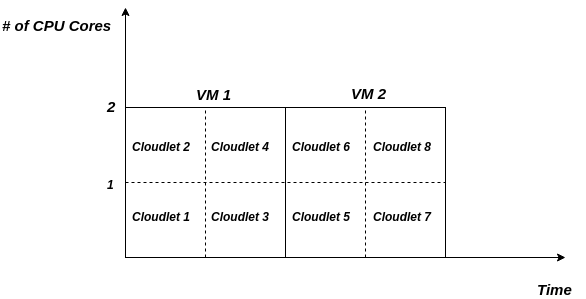
\includegraphics[scale=0.4]{space_vm_space_cloudlet.png}
\caption{Space Shared Allocation Policy for VMs and Cloudlets}
\end{figure}




\newpage
\bibliographystyle{IEEEtran}
\bibliography{ref}



\end{document}